\documentclass[a4paper]{report}
    
    %% Language and font encodings
    \usepackage[english]{babel}
    \usepackage[utf8x]{inputenc}
    \usepackage[T1]{fontenc}
    
    %% Sets page size and margins
    \usepackage[a4paper,top=3cm,bottom=2cm,left=3cm,right=3cm,marginparwidth=1.75cm]{geometry}
    
    %% Useful packages
    \usepackage{url}
    \usepackage{amsmath}
    \usepackage{graphicx}
    \usepackage[colorinlistoftodos]{todonotes}
    \usepackage[colorlinks=false, allcolors=blue]{hyperref}
    \usepackage[acronym]{glossaries}
    \usepackage{acronym}
    \usepackage{amssymb}
    
    
    \title{Random Forest}
    \author{Timo Blust\\[1cm]{\small Supervisor: Dr. Ing. A. Laubenheimer}}
    
    \begin{document}
    \maketitle
    \tableofcontents
    
    \chapter{Introduction to machine learning}
    
    Nowadays there exist hundreds (or even thousands) of different algorithms that are classified as machine learning algorithms. But what classifies an algorithm (or a program) as a machine learning algorithm (or program)? Probably the most popular definition of machine learning was provided by Tom Mitchell in 1997: ``A computer program is said to learn from experience $E$ with respect to some task $T$ and some performance measure $P$, if its performance on $T$, as measured by $P$, improves with experience $E$.'' \cite{mitchell97}.
    A very popular example of such a program is DeepMind's AlphaGo \cite{alphago}. AlphaGo is a computer program that learns to play the ancient Chinese board game Go \cite{go}. For the definition above, this means that the task $T$ is playing Go (whether against itself or a human player), the experience $E$ is the data of all previously played games and the performance measure $P$ simply decides if a game is won or lost. If the program is a machine learning program, it has to improve over time (more formal: over the amount of played games). This means the more games the program played, the more likely it is to win its next game.
    
    \section{Learning types}
    
    Machine learning algorithms are divided into four sub-classes:
    \begin{itemize}
    \item Supervised learning
    \item Unsupervised learning
    \item Semi-supervised learning
    \item Reinforcement learning
    \end{itemize}
    
    \subsection{Supervised learning}
    \label{sec:supervised-learning}
    In supervised learning, the learner (that is the training algorithm) tries to approximate a function $f(x) = Y$ from labeled training data. The training data is a set of examples. An example consists of an input $x$ (typically a n-dimensional vector) and its desired output $Y$ (the label) \cite{supervised-learning}. The accuracy of algorithms that use supervised learning techniques can be measured by the ratio of correct predictions to the total amount of predictions during testing.
    
    A popular example of supervised learning is the task of detecting handwritten digits. The MNIST \cite{mnist} database contains 70,000 labeled images (28x28 pixel) for training and testing supervised learning algorithms. In this example the input vector $x$ is an (flattened) image and its desired output $Y$ is the digit, that is represented in the image given by $x$.
    Popular supervised learning algorithms are support vector machines, linear regression, decision trees and neural networks.
    
    \subsection{Unsupervised learning}
    Like in supervised learning, unsupervised learning is the task of approximating a function $f(x) = Y$. However, in unsupervised learning $Y$ (the output or label) is unknown and not given in the training set. Hence, accuracy measurement is also impossible. Algorithms like k-means, generative adversarial networks (a sub-class of neural networks) or anomaly detection are unsupervised \cite{unsupervised-learning}.
    
    \subsection{Semi-supervised learning}
    As the name suggests, semi-supervised learning combines the two methods mentioned previously. Semi-supervised learning tries to accomplish supervised learning tasks with a training set of which the majority of the data points are unlabeled \cite{semi-supervised-learning}. Typically, labeling data requires expert knowledge and time which can lead to high costs in real world applications. Semi-supervised learning splits in two classes:
    \begin{itemize}
    \item transductive learning: the algorithm tries to find the labels for all unlabeled examples in the training set only,
    \item inductive learning: the algorithm tries to learn a general rule that can map the entire input set to the output set.
    \end{itemize}
    
    \subsection{Reinforcement learning}
    Unlike any of the previously mentioned methods, \ac{RL} does not require a training or testing data set at all \cite{reinforcement-learning}. In \ac{RL}, the agent (that is the specific \ac{RL} algorithm) has three major differences to the previously mentioned \acl{ML} techniques:
    \begin{itemize}
    \item it does not require any training or testing data,
    \item it interacts with its environment (meaning it can influence its own input data),
    \item it is a reward based system (meaning it can be rewarded/punished for good/bad decisions).
    \end{itemize}
    Learning is achieved by applying the agent to its environment. The task of the agent is then to decide which action (from the set of all possible actions) should be executed at the current circumstances (the state of the agent itself, as well as the state of the environment) in order to maximize the total future reward. After this action has been executed, the environment forwards the new state and the current reward back to the agent. This agent-environment interaction loops until a goal state is reached \cite{reinforcement-learning-silver15}. 
    Games are usually good environments for \ac{RL} agents. An agent is trained to play a certain game. The game reports its state (for example: how many enemies are there and where are they, are there any obstacles around the player, ...) and the current reward (for example: the player's score) to the agent. Now the agent has to choose an action for the next step/iteration of the loop (for example: move left/right/top/bottom, jump, hide, ...). This action is then applied to the environment. The goal state is reached, if the game ends (for example: all enemies are defeated, all coins are collected, time is over, ...). 
    
    \section{Classification and regression}
    
    Supervised learning tasks can be divided even further into the categories \textit{classification} and \textit{regression}.
    The difference between the both classes is the kind of prediction they make \cite{class-and-regr}.
    
    In \textit{classification} the output (prediction) is categorical. The MNIST \cite{mnist} data set, for example, addresses a classification problem. The classifier (that is the function that is used to classify or label the data) takes an image as an input and returns the most likely category (digits from 0 to 9) of that image. If one passes a random image (that does not contain a digit at all) as an input, like a photo of a mountain, the classifier will still categorize the image as some digit (whether this makes sense or not).
    
    In \textit{regression} the output (prediction) is continuous. Predicting the market price of a house, for example, is a regression problem. The regressor (that is the function that produces the output value) takes some sort of input data (like price history and data about the property market) and predicts the house's price in a year. The price could, theoretically, be any number and is therefore continuous.
    
    \chapter{Decision Tree}
    
    \begin{figure}[h]
    \centering
    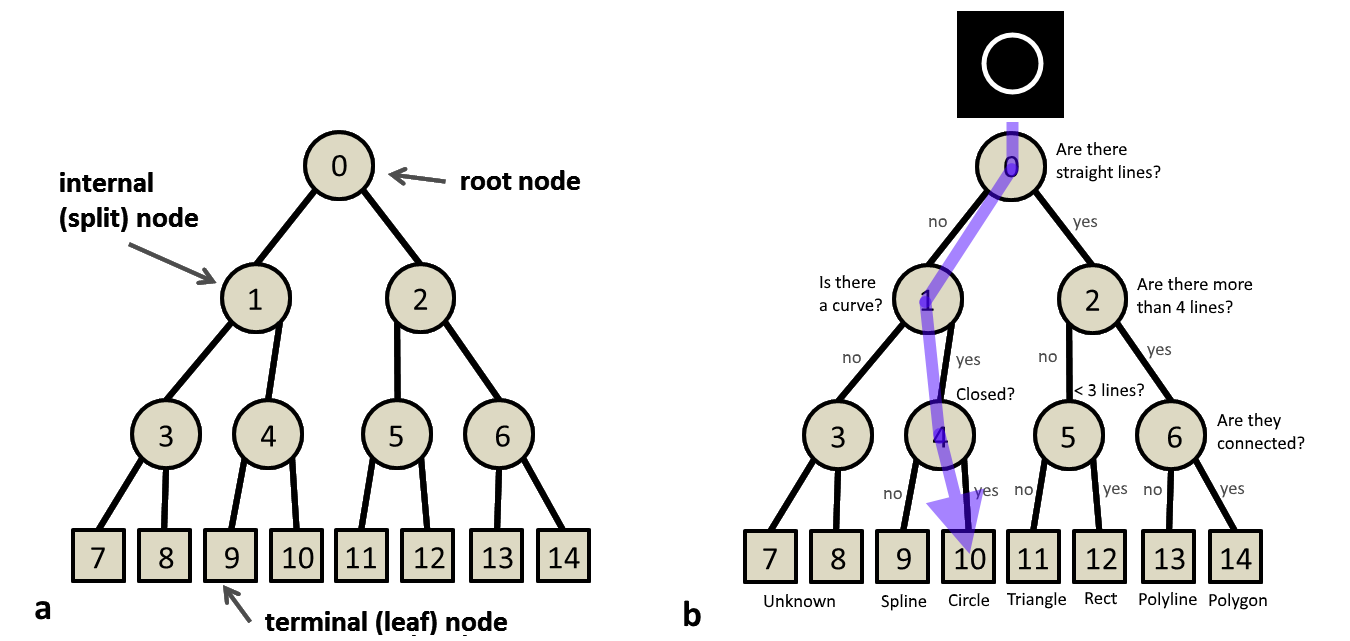
\includegraphics[width=\textwidth]{decisiontree}
    \caption{\textbf{Binary decision tree. (a)} Trees are hierarchical structures consisting of nodes and edges. In contrast to graphs, trees do not have loops. \textbf{(b)} Example decision tree that detects primitive geometries in an image. }
    \label{fig:dtree}
    \end{figure}
    
    The basic elements of random forests are decision trees (like in nature: a collection of trees is called forest). ``A tree is a collection of nodes and edges organized in a hierarchical structure [...]. Nodes are divided into internal (or split) nodes and terminal (or leaf) nodes.'' \cite[p.6]{ms11}. \textit{Decision} trees are used to make decisions about certain criteria. 
    
    In a decision tree, each split node represents a decision (or test) and each edge the outcome of the previous decision. Figure \ref{fig:dtree}b shows an example decision tree. This tree tries to classify the shape of a given geometry (from a binary image, for example). The decision making starts at the top (root) node and continues level-wise (top-down) until it reaches a leaf node.
    
    How does a decision tree know which decision belongs to the root node and which decisions have to follow which outcomes (from previous decisions)? 
    
    \section{Building a decision tree}
    
    For an easier understanding of decision trees an example environment is introduced.
    
    \subsubsection{Example: toy production line}
    Imagine a company that produces toys (like action figures). At the end of the production process, a large conveyor belt has to transport all the different toys to their place in the warehouse. The company did not tag the toys when they were produced (with a bar code or similar) and now the automatic storage system cannot distinguish the toys from each other. To resolve this problem, some sort of classification system is attached to the conveyor belt. This classification system is now responsible for telling the storage system of which type each toy is, so that the storage system can store the toys at the right places in the warehouse.
    The production line provides the eight different toys given in image~\ref{fig:collection}.
    
    \begin{figure}
    \centering
    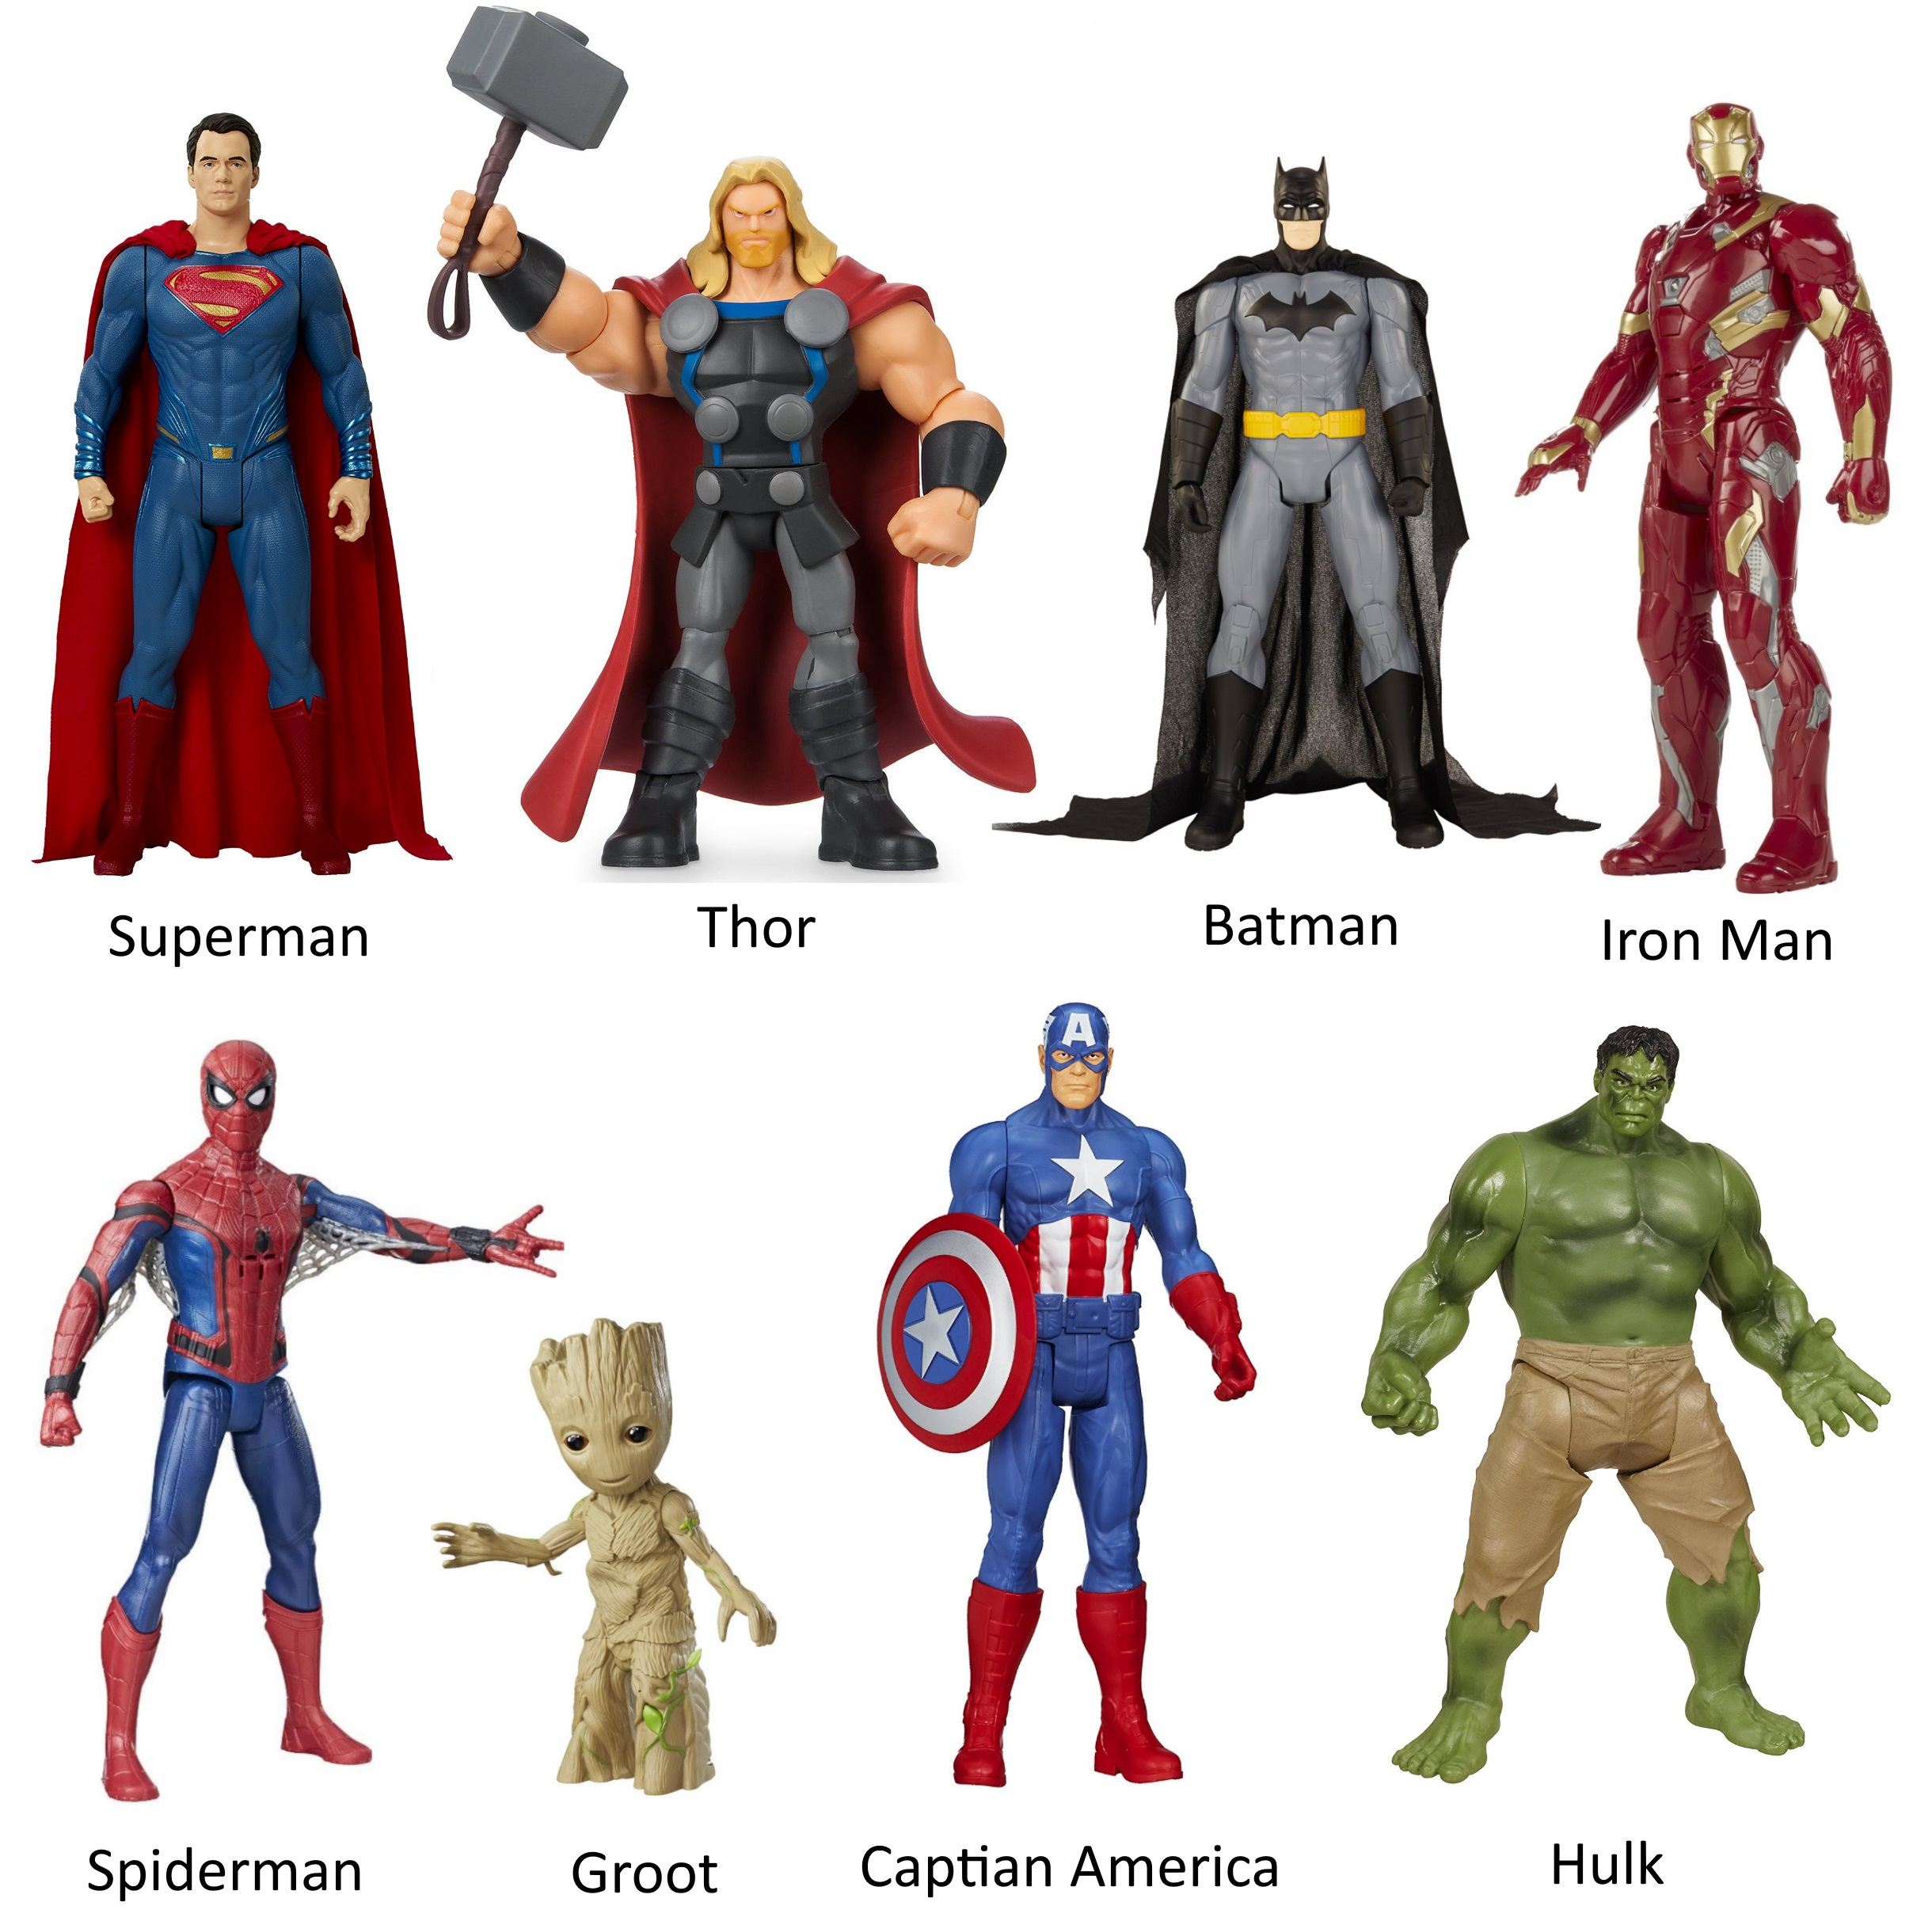
\includegraphics[width=0.5\textwidth]{collection}
    \caption{\textbf{Toy production line.} The toys produced by the company in the example.}
    \label{fig:collection}
    \end{figure}
    
    A top of the art computer vision system is integrated in the classification system and feeds it with different features (gained from multiple cameras that take pictures of each toy on the conveyor belt). The computed features are:
    \begin{itemize}
    \item body shape $x_1\in\{humanoid, unknown\}$
    \item main color $x_2\in\{red, blue, green, brown, gray, yellow, purple, white, black\}$
    \item accessory 1 $x_3\in\{cape, hammer, shield, mask, net, nothing\}$
    \item accessory 2 $x_4\in\{cape, hammer, shield, mask, net, nothing\}$
    \item height $x_5=[1, 10]$ (cm)
    \end{itemize}
    The classification system has then to decide (based on the given features) of which type each toy is. A decision tree is used as the decision maker. Valid decisions $Y$ are \textit{Superman, Thor, Batman, Iron~Man, Spiderman, Groot, Captain~America} and \textit{Hulk}
    
    Before the decision tree can be used, it has to be trained with a set of training data. Because a decision tree is a supervised learning model, the training set must be labeled (see section \ref{sec:supervised-learning}). An example in a training set is denoted as \[\textbf{s}=(\textbf{x},Y)=\{x_1, x_2, ..., x_d, Y\}\] where $d$ is the dimensionality of the input vector $\textbf{x}$ (5 in the toy company example) and $Y$ the desired label (or class) of an input vector. Each feature (or attribute) in the input vector ($x_1, ..., x_d$) can either be discrete or continuous, depending on the training algorithm. In the toy company example there are four discrete ($x_1, ..., x_4$) and one continuous ($x_5$) attributes.
    
    For instance, a sample training set (or at least a few entries of it), that could be used to build the tree in figure \ref{fig:dtree}b is given in table \ref{tab:training-sample}
    \begin{table}
    \centering
    \begin{tabular}{ |c|c|c|c|c||c| }
    \hline
    body shape $x_1$ & main color $x_2$ & accessory 1 $x_3$ & accessory 2 $x_4$ & height $x_5$ & type $Y$\\
    \hline
    humanoid & red & net & mask & 9 & Spiderman \\
    humanoid & blue & cape & nothing & 10 & Superman \\
    humanoid & gray & cape & hammer & 9 & Thor \\
    humanoid & cape & mask & gray & 10 & Batman \\
    humanoid & red & mask & nothing & 10 & Iron Man \\
    humanoid & brown & nothing & nothing & 6 & Groot \\
    humanoid & blue & net & mask & 10 & Spiderman \\
    humanoid & blue & mask & nothing & 9 & Spiderman \\
    \hline
    \end{tabular}
    \caption{\textbf{Sample training set.} A possible (part of a) training set for the decision tree in the toy company example. $x_1$ to $x_4$ are discrete attributes while $x_5$ is continuous.}
    \label{tab:training-sample}
    \end{table}
    
    \subsection{Information theory}
    In order to understand decision tree learning, one has to understand the meaning of entropy and information gain.
    
    \subsubsection{Entropy}
    Entropy is a measure of impurity of a distribution of a random variable. In the case of training a \acs{ML} model, like a decision tree, the random variable refers to a feature (column) in the training set. The \textit{has curves} feature in table \ref{tab:training-sample} for instance, can take one of two values (\textit{true} or \textit{false}) and contains 7 samples. The distribution of this feature is 3 times \textit{true} and 4 times \textit{false}, which means that the variable is fairly even distributed. An even distribution yields a high entropy which indicates that the distribution is impure.
    
    For a discrete random variable $X \in \{x_1, ..., x_n\}$ entropy is defined as \[H(X)=-\sum_{i=0}^{n}P(x_i)log_2P(x_i)\]
    $P(x_i)=[0, 1]$ is the probability of $X$ being $x_i$ in a randomly selected sample. The logarithmic part of the equation applies a weight to the probability, depending on the probability itself. Because $\lim_{x \to 0}log_b(x)=-\inf$ for $x\in\mathbb{R}^+$ and $log_b(1)=0$ for any base $b$, the weight of values with high probability is smaller than the weight of values with low probability. As a result, sparse distributed distribution (only a few values with high probability) yield lower entropies than high distributed distributions. Figure~\ref{fig:entropy} illustrates the entropy for different distributions.
    
    \subsubsection{Gini impurity}
    A similar alternative to entropy is the gini impurity which is defined as $$Gini(X)=1-\sum_{i=0}^{n}P(x_i)^2$$
    The behavior of both, entropy and gini impurity, is identical in the matter of indicating impurity. Both functions fall if the distribution maximizes its purity and rise if the distribution maximizes its impurity. However, there can be a computational advantage of gini due to the replacement of the log function with a simple multiplication \cite{log-complexity}.
    
    \subsubsection{Information gain}
    Information gain 
    
    \begin{figure}
    \centering
    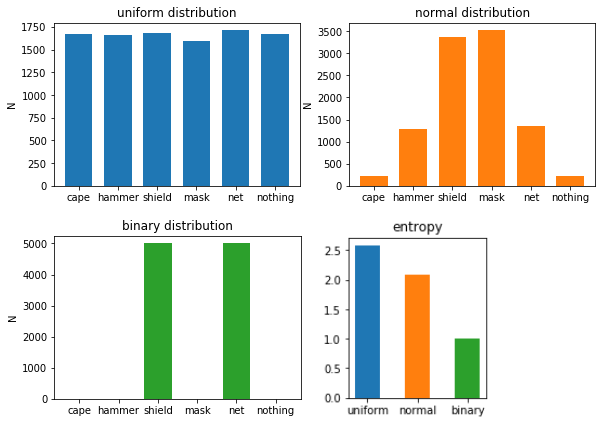
\includegraphics[width=\textwidth]{entropy}
    \caption{\textbf{Distributions and their entropies.} Three different distributions (uniform, normal and binary on a set with 10000 samples) of the \textit{accessory} attribute in the toy company example. The bottom right chart shows the entropy for each distribution. The less distributed the set is, the lower is the entropy. }
    \label{fig:entropy}
    \end{figure}
    
    \subsection{ID3}
    
    
    \chapter*{Acronyms}
    \begin{acronym}	
        \acro{ML}{machine learning} 
        \acro{RL}{reinforcement learning} 
           %\acro{CV}{computer vision} 
    
    \end{acronym}
     
    \bibliographystyle{ieeetr}
    \bibliography{sources}
    
    \end{document}